\documentclass{endm}
\usepackage{endmmacro}

\usepackage[paper=a4paper, left=1.5cm, right=1.5cm, bottom=1.5cm, top=3.5cm]{geometry}
\usepackage[utf8]{inputenc}
\usepackage[spanish,es-nodecimaldot]{babel}
\usepackage{graphicx}
\graphicspath{ {imagenes/} }

\begin{document}

% CARATULA
\begin{frontmatter}

\title{Trabajo Práctico 3}

\author{Fuerte A Pachi}
\address{Frachtenberg Goldsmit, Kevin\\ Mena, Manuel\\ Szperling, Sebastián\\ Tarrio, Ignacio}

\author{Métodos Numéricos}
\address{2do Cuatrimestre, 2017\\ Facultdad de Ciencias Exactas y Naturales\\ Universidad de Buenos Aires\\ Buenos Aires, Argentina}

\begin{abstract}
\end{abstract}

\end{frontmatter}

\newpage
\tableofcontents

\newpage
\section{Introducción}

El presente trabajo práctico consiste en aplicar técnicas de Métodos Numéricos y Data Science, en particular Regresiones Lineales con Cuadrados Mínimos sobre un gran conjunto de datos buscando proveer información descriptiva y de modelos que puedan ser utilizados para predecir fenómenos que afecten a la puntualidad (OTP), pero no necesariamente limitados a ésta.

Los datos a analizar comprenden cierta información relacionada a vuelos realizados en Estados Unidos entre los años 1987 y 2008, incluyendo información de la compañía, fecha y horarios planificados de partida/arribo, horarios reales de salida/llegada, causa del delay, si fueron cancelados o no, y su respectiva causa, el tipo de avión utilizado, tiempo de vuelo, tiempos de taxi, entre otras cosas. Para mas detalle puede consultarse http://stat-computing.org/dataexpo/2009/the-data.html .%PONER COMO LINK

Se tuvo en cuenta distintas funciones para predecir y se analizó cuál predice mejor utilizando una parte de los datos como entrenamiento y la otra para comparar con lo predicho. El criterio de comparacion entre funciones es analizar el ECM (Error cuadrático medio) de lo predicho con lo real.

% Complicacion con la semana 53, usamos 



\newpage
\section{Vuelos por mes}

Para el primer análisis se decidió observar la cantidad de vuelos por mes entre los años 2003 y 2008. En el caso de lograr una predicción ajustada, esta información podría ser utilizada para calcular insumos necesarios en los próximos años dependiendo de la cantidad de vuelos que se realizarán.

\subsection{Primeras hipótesis y bases del análisis}

Nuestra hipótesis respecto de este eje es que la cantidad de vuelos de cada aeropuerto debería aumentar a lo largo de los años dado que el tráfico áereo aumenta a la par. Los experimentos comprenden a todos los aeropuertos.

Consideramos los datos a partir del año 2003 debido al incidente de 2001 previamente mencionado.

Una observación al respecto de este gráfico es que en todos los años, febrero tiene un pico bajo de vuelos. No pudimos encontrar la razón por la cual sucede esto, lo único que pudimos observar es que esa fecha coincide con el intervalo de clases entre dos períodos de vacaciones: el president’s day y spring break.

\subsection{Datos concretos y estimaciones}

Para realizar los gráficos se acumuló por cada mes de cada año la cantidad de vuelos sucedidos. La función utilizada con CML para esta estimación fue:

\smallskip

$y(x) = ax + b|cos(x)| + c|sin(x)| + d \times log(x+1) + e + f \times cos(x) + g \times sin(x) + hx^4 + ix^3 + jx^2$

Uno de los experimentos realizados fue variar los años de entrenamiento y estimar los siguientes años. Se comparó un conjunto entrenado con un año extra que el resto para comprobar si la diferencia en la precisión era sustancial o no. La hipótesis es que al haber entrenado con una mayor cantidad de datos, es posible dar una mejor predicción de los siguientes años, pero podría ser posible que esto no ocurriese así sino que durante ese año extra la disposición de los datos sea muy particular y que se produzca el fenómeno de overfitting, resultando en una predicción de menor calidad.

Estos son los resultados de entrenar a la función entre los años 2003 y 2006, prediciendo de 2006 a 2008.

\begin{figure}[!htb]
\begin{center}
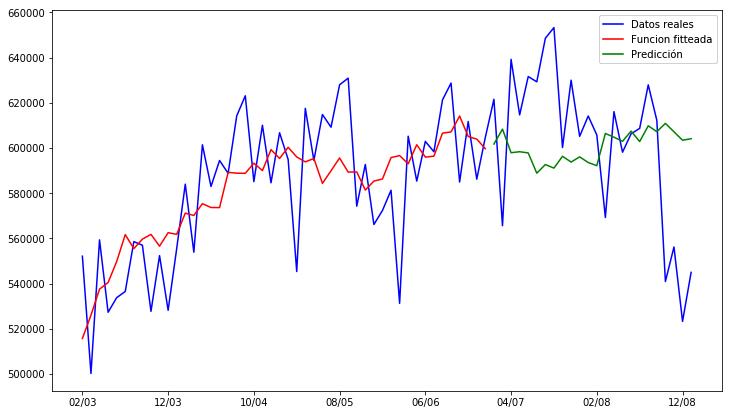
\includegraphics[scale=0.5]{vuelos_3-6_7-8.png}
\caption{caption}
\label{vuelos-1}
\end{center}
\end{figure}

El error cuadrático medio para estas estimaciones fue de 840810926.93.

Luego se experimentó tomando distintos rangos de entrenamiento: 2003-2005, 2004-2006 y 2005-2007, prediciendo 2005-2006, 2006-2007 y 2007-2008, respectivamente.

\begin{figure}[!htb]
\begin{center}
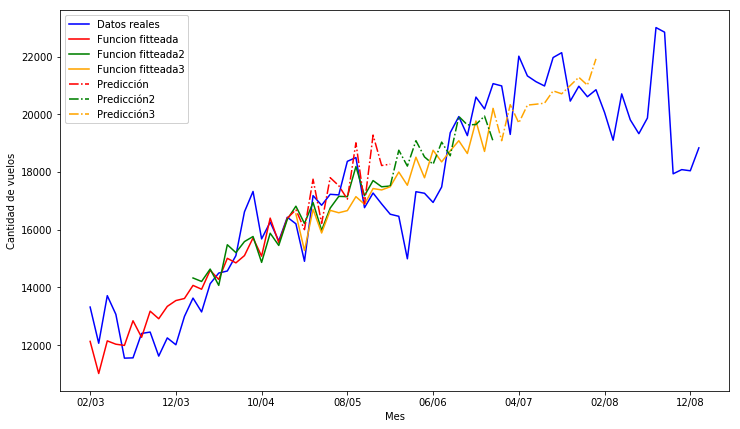
\includegraphics[scale=0.5]{vuelos_multiples.png}
\caption{caption}
\label{vuelos-2}
\end{center}
\end{figure}

Los EMC fueron 11228017738.2, 1215421229.42, 1214577235.23, según el orden en que los rangos están dispuestos.

Como puede observarse, el EMC para la función entrenada desde 2003 a 2006 es mucho menor que el resto, y esto se cree que se debe a ese año extra que tiene de entrenamiento.


\subsection{ECM de funciones de predicción}

Otra experimentación realizada fue la comparación de los ECM entre distintas funciones de predicción. Se crearon 6 funciones distintas listadas a continuación, de las cuales una es una función lineal y las otras pertenecen a la familia de funciones trigonométricas.

En todas las funciones que corresponden, las letras entre \textit{a} y \textit{l} fueron los parametros que se ajustaron con el entrenamiento, el cual fue dado con la información de los años 2003 a 2006 y luego se procedió a predecir los años 2007 y 2008.

\begin{enumerate}
  \item $y(x) = a + bx$
  \item $y(x) = ax + b|cos(x)| + c|sin(x)| + f  \times  cos(x) + g  \times  sin(x) + d  \times  log(x+1) + e$
  \item $y(x) = hx^4 + ix^3 + jx^2 + ax + b|cos(x)| + c|sin(x)| + f  \times  cos(x) + g  \times  sin(x) + d  \times  log(x+1) + e$
  \item $y(x) = ax + b|cos(x)| + c|sin(x)| + f  \times  cos(x) + g  \times  sin(x) + d  \times  log(x+1) + e + k  \times  sin(x) ^ 2 + l  \times  cos(x) ^ 2$
  \item $y(x) = ax + b|cos(x)| + c|sin(x)| + f  \times  cos(x) + g  \times  sin(x) + d  \times  cos(x) + i  \times  sin(x)  + e$
  \item $y(x) = a + bx + c  \times  cos(xd + e) + f  \times  sin(xg + h) + c  \times  cos(xd + e) + f  \times  sin(xg + h)$
\end{enumerate}


Como hipótesis de este experimento se planteó que la función lineal (1) sería la que mayor error cuadrático medio tendría ya que es la que menor cantidad de parámetros tiene y además es poco flexlible. Dado que las otras 5 funciones pertenecen a la misma familia de funciones, se esperó que éstas tengan un comportamiento similar.

Una vez ejecutado las pruebas, los errores que se obtuvieron para cada función fueron los siguientes:

\begin{figure}[!htb]
\begin{center}
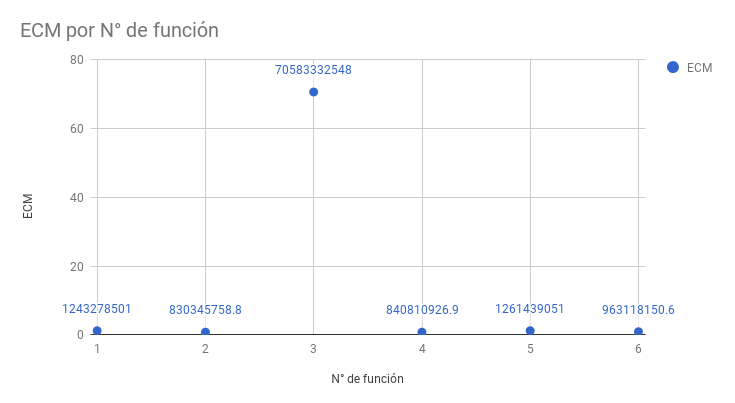
\includegraphics[scale=0.5]{imagenes/ecm_por_fn.png}
\caption{caption}
\label{vuelos-3}
\end{center}
\end{figure}

Se pudo observar con el anterior gráfico cómo la función número 3 fue la que mayor error cuadrático medio obtuvo y por mucha diferencia a pesar de ser de la misma familia de funciones que las demás (sin contar la función lineal) y de tener la misma cantidad de parámetros que la función número 5. También se observó que la función lineal a pesar de estar muy por debajo que la función 3, estuvo solo un poco por debajo que la función 5 y aun así se mantuvo por encima de las otras 3 funciones.
La función que menor ECM obtuvo fue la función número 4, la cual fue la que mayor cantidad de parametros ajustables tenía.

\section{Demoras por mes y distancia}

Decidimos analizar cómo se relacionan las demoras y la distancia del vuelo. Estas demoras tienen distintas causas, prestamos atención a las que están representadas en los dato, quedándonos con las siguientes tipos de demora:
\begin{itemize}
\item Aerolínea (problemas de mantención del avión, o de los empleados)
\item Mal clima
\item NAS(National Aviation System, demoras causadas por operaciones del aeropuerto, tráfico voluminoso y/o control del tráfico aéreo)
\item Avión retrasado (demora por un vuelo anterior llegando tarde, causando que el vuelo presente salga más tarde)
\item Seguridad
\end{itemize}

\subsection{Primeras hipótesis y bases del análisis}

Nuestra hipótesis respecto a este eje es que la causas de demoras afectan a los tipos de vuelo por igual, ya que las causas anteriormente nombradas no parecerían tener algún tipo de relación con la distancia del vuelo.

Para estos experimentos utilizamos los datos entre los años 2003-2008 (no hay información para años previos). 

%-Grafico 1
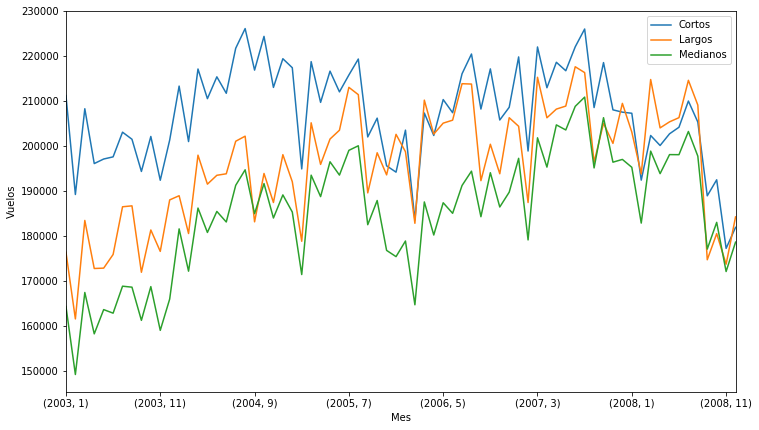
\includegraphics[scale=0.9,natwidth=732,natheight=415]{distancia1.png}

Podemos ver como la cantidad de vuelos según tipo es bastante similar, y escala muy parecido en el tiempo, salvo los vuelos cortos que sufre una caída más notoria a partir del 2008.

%-Grafico 2
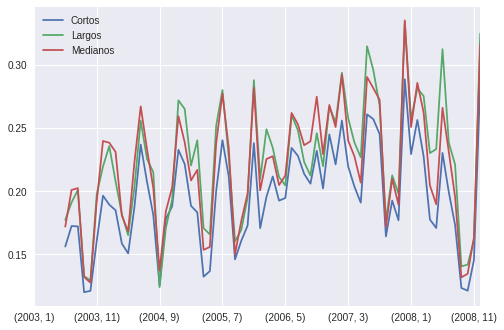
\includegraphics[scale=0.9,natwidth=732,natheight=415]{distancia2.png}

En este segundo gráfico notamos, primero que el porcentaje es muy similar para las 3 categorías, hay menos vuelos retrasos en vuelos cortos, posiblemente debido a que necesitan una menor preparación, aunque no es una diferencia significativa. Y otra dato que extrajimos de este gráfico es que las demoras son estacionarias, y tienen una frecuencia bastante regular ya que podemos notar que los altibajos se producen en las mismas épocas del años para los distintos tipos. Por esto prestaremos atención al estimar a los senos y cosenos.


\subsection{Datos concretos y estimaciones}

Primero queríamos ver cómo responden las estimaciones, así que siguiendo el approach anterior, estimamos el porcentaje de demoras para vuelos medianos, tratando de estimar 2006, 2007 y 2008, para cada año tomamos los dos años anteriores

%Grafico 3 y 4
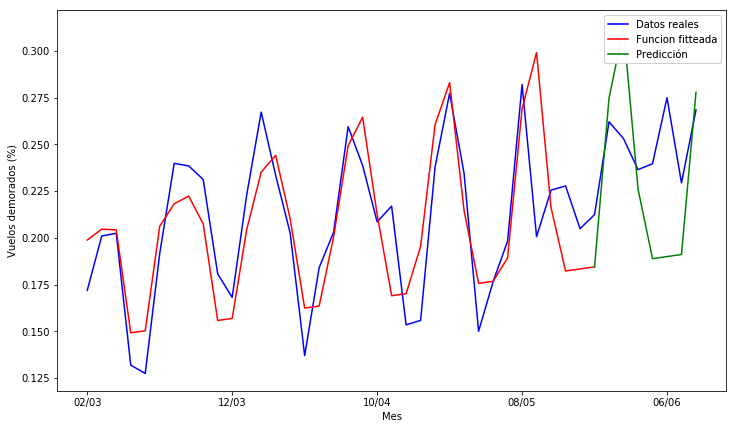
\includegraphics[scale=0.9,natwidth=732,natheight=415]{distancia3.png}
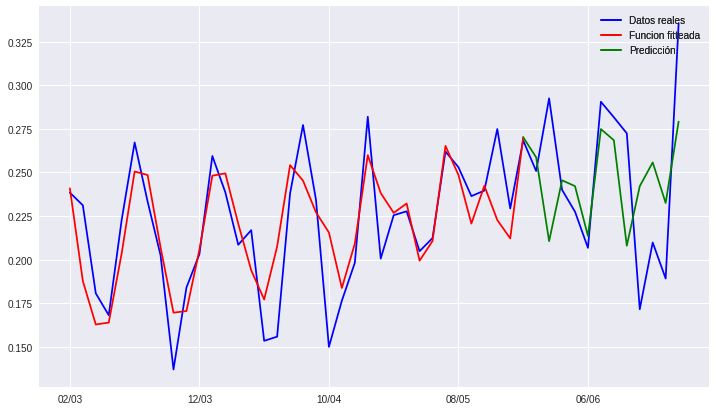
\includegraphics[scale=0.9,natwidth=732,natheight=415]{distancia4.png}

Los errores cuadráticos medios para estas estimaciones fueron 0.001143 (izquierda), y 0.001758 (derecha). La función utilizada con CML para esta estimación fue:

\bigskip

$f(x) = a + bx + c \times cos(xd + e) + f \times sin(xg + h) + i$

La intuición que tuvimos para encontrar la función fue usar cosenos y senos por la frecuencia y amplitud de los datos.

Este otro experimento consistió en reutilizar los parámetros obtenidos por el método en el tipo de vuelo anterior y tratar de estimar el porcentaje de demoras para vuelos largos.

%Grafico 5
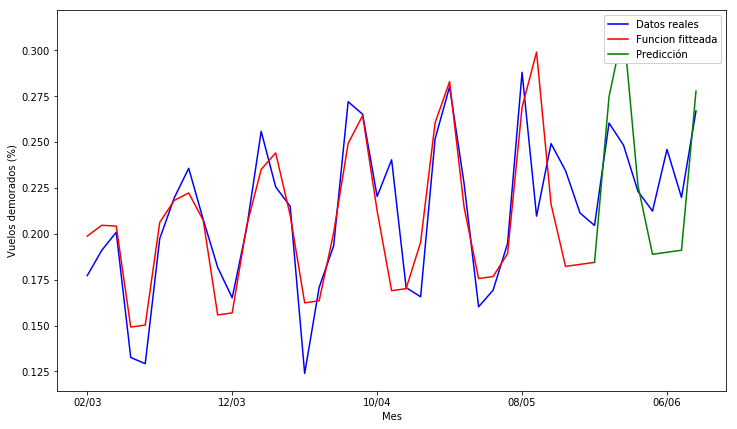
\includegraphics[scale=0.9,natwidth=732,natheight=415]{distancia5.png}

Como se puede observar la predicción se comporta bastante parecida a los datos reales, esta se acopla muy bien a la frecuencia, pero en el 2007 se puede observar una amplitud de los datos más pequeña que los años anteriores y ahí es donde más falló la estimación.

\newpage
\section{Conclusión}

En cuanto a cantidad de vuelos por año pudo observarse un aumento a lo largo del tiempo. La precisión de las predicciones se vio afectada por unos outliers periódicos que ocurren cada febrero, estos elevan el error cuadrático medio creando una disrupción en el entrenamiento y por ende, en la predicción. También se observó que un entrenamiento de mayor rango trae mejores resultados en la predicción pero como los vuelos pueden estar afectados por factores externos e impredecibles, es posible que un rango demasiado grande resulte perjudicial, como podría ser el caso de tomar como parte del entrenamiento los vuelos durante los años 2001 y 2002 donde la cantidad de vuelos se ve comprometida por los eventos sucedidos.

Es importante tener en cuenta la naturaleza de la información a manejar. Se llegó a la conclusion de que es necesario tener cautela qué porción de los datos elegir para ser tenida en cuenta. El conocimiento y análisis en la información disponible permite poder ajustar lo mejor posible el entrenamiento, conociendo los datos es posible llegar a una mejor discriminación de cuales son outliers y cuáles no para que pueda resultar en una predicción más acertada.

En este caso conocer que se trata de vuelos dentro de Estados Unidos permite realizar algunas suposiciones que merecen ser tenidas en cuenta a la hora de predecir, como por ejemplo, que la cantidad de vuelos pueda ir en aumento pero se vea obstaculizada por factores que todavía no hacen efecto en el conjunto de datos pero que pueden estar presentes como la saturación del espacio aéreo o la capacidad de los aeropuertos.

Por otro lado, en cuanto a la demora de vuelos se observó que entre los años 2003 y 2005 se producían cambios similares, pero que a partir de ese último año las demoras ocurridas mostraron un patrón diferente, lo cual causaría que el entrenamiento realizado con los primeros años falle en la predicción. Sin embargo se obtuvo una predicción cercana a los hechos reales a causa de la función utilizada para predecir y de haber tenido en cuenta el origen de los datos y su comportamiento en general.

El hecho de tener en cuenta el origen y el comportamiento de los datos está basado en la hipótesis planteada, en la cual se propuso que las causas de demora afectan todas por igual y luego de haber realizado las experimentaciones pertinentes, se concluyó que la hipótesis era correcta para la predicción de demoras en los vuelos.

% compilar 2 veces para actualizar las referencias


\end{document}